\documentclass[11pt]{article}

\usepackage[margin=1in]{geometry}
\usepackage{setspace}
\onehalfspacing
\usepackage{graphicx}
\graphicspath{report_images/}
\usepackage{appendix}
\usepackage{listings}
\usepackage{float}
\usepackage{multirow}
\usepackage{amsthm}
% The next three lines make the table and figure numbers also include section number
\usepackage{chngcntr}
\counterwithin{table}{section}
\counterwithin{figure}{section}
% Needed to make titling page without a page number
\usepackage{titling}

% DOCUMENT INFORMATION =================================================
\font\titleFont=cmr12 at 11pt
\title {{\titleFont ECEN 429: Introduction to Digital Systems Design Laboratory \\ North Carolina Agricultural and Technical State University \\ Department of Electrical and Computer Engineering}} % Declare Title
\author{\titleFont Reporter: Chris Cannon \\ Partner: Nikiyah Beulah} % Declare authors
\date{\titleFont April 5, 2018}
% ======================================================================

\begin{document}

\begin{titlingpage}
\maketitle
\begin{center}
	Prelab 9
\end{center}
\end{titlingpage}

\section{Introduction}
The purpose of this prelab is to evaluate the state machine involved in a Traffic Light Controller.

\section{Background, Design Solution, Results}
\subsection{Problem 1}
What are the states within the FSM? What happens in each state?

The 3 bits in NS represent red, yellow, and green lights, respectively.
The 3 bits in EW represent red, yellow, and green lights, respectively.

\begin{figure}[H]
\begin{center}
	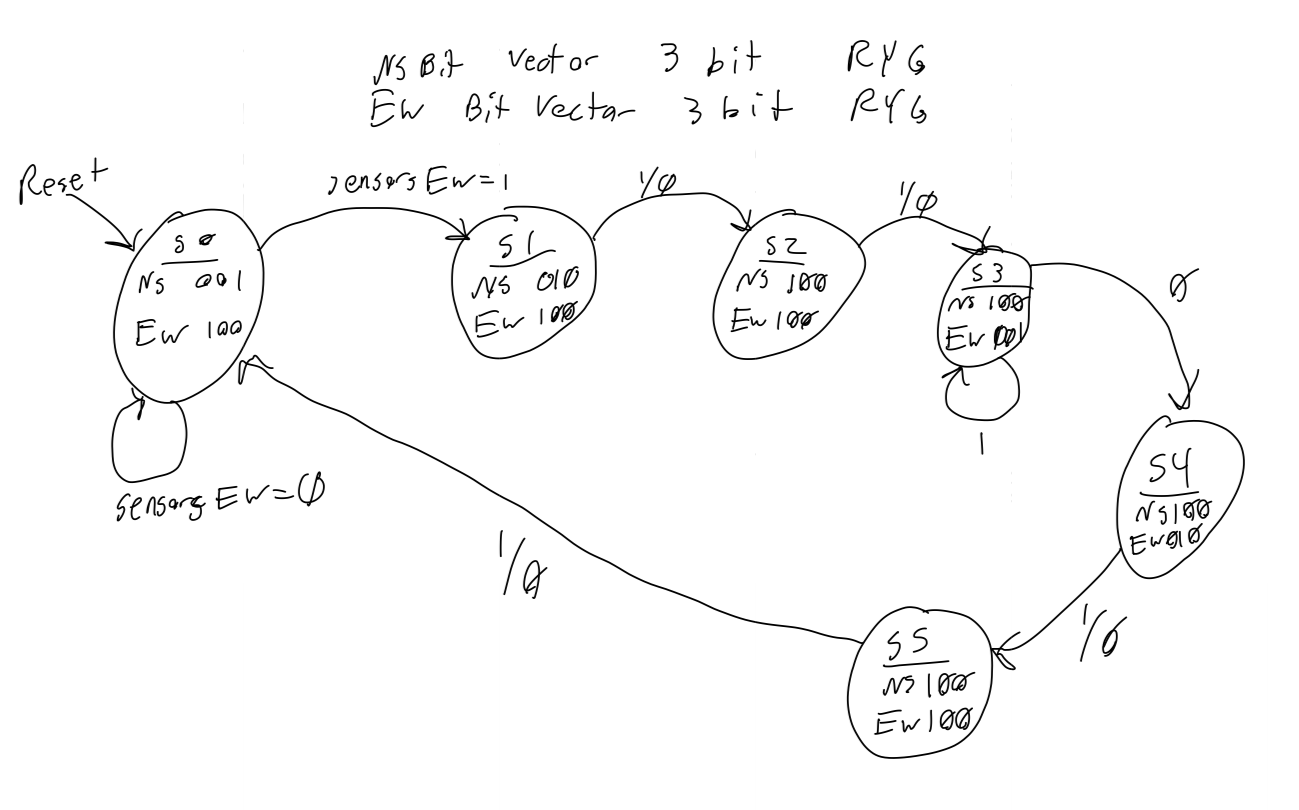
\includegraphics[width=\textwidth]{./9images/trafficLight.png}
	\caption{\label{fig:trafficLight} State Machine for traffic light}
\end{center}
\end{figure}

\subsection{Problem 2}
Add turn lanes for the N/S direction (when traveling from North to South) only. Design a new FSM that accounts for this (includes the turn signal within the cycle). 

The 5 bits in NS represent red, yellow, yellow flashing arrow, green and green arrow lights, respectively.
The 3 bits in EW represent red, yellow, and green lights, respectively.

\begin{figure}[H]
\begin{center}
	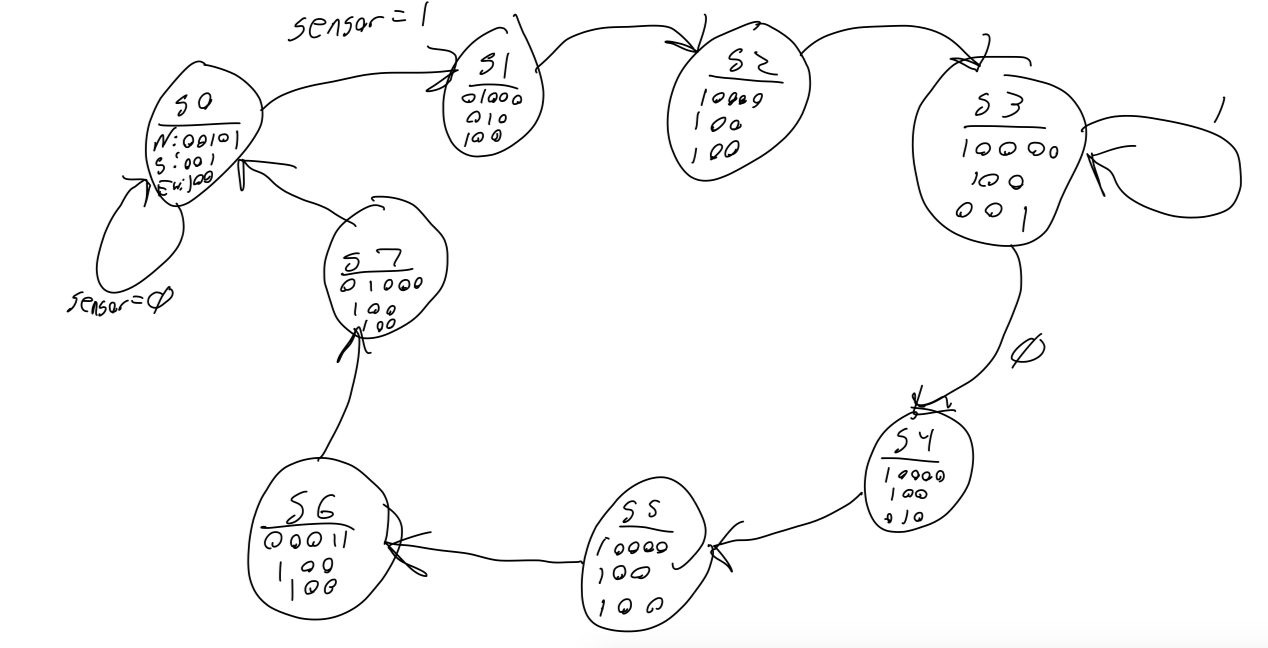
\includegraphics[width=\textwidth]{./9images/trafficLightWithTurn.png}
	\caption{\label{fig:trafficLightWithTurn}State Machine for traffic light with a turn lane}
\end{center}
\end{figure}

\subsection{Problem 3}
Add a sensor for the turn lane (it only turns on when a car is present). Design a new FSM that accounts for this.

The 5 bits in NS represent red, yellow, yellow flashing arrow, green and green arrow lights, respectively.
The 3 bits in EW represent red, yellow, and green lights, respectively.

\begin{figure}[H]
\begin{center}
	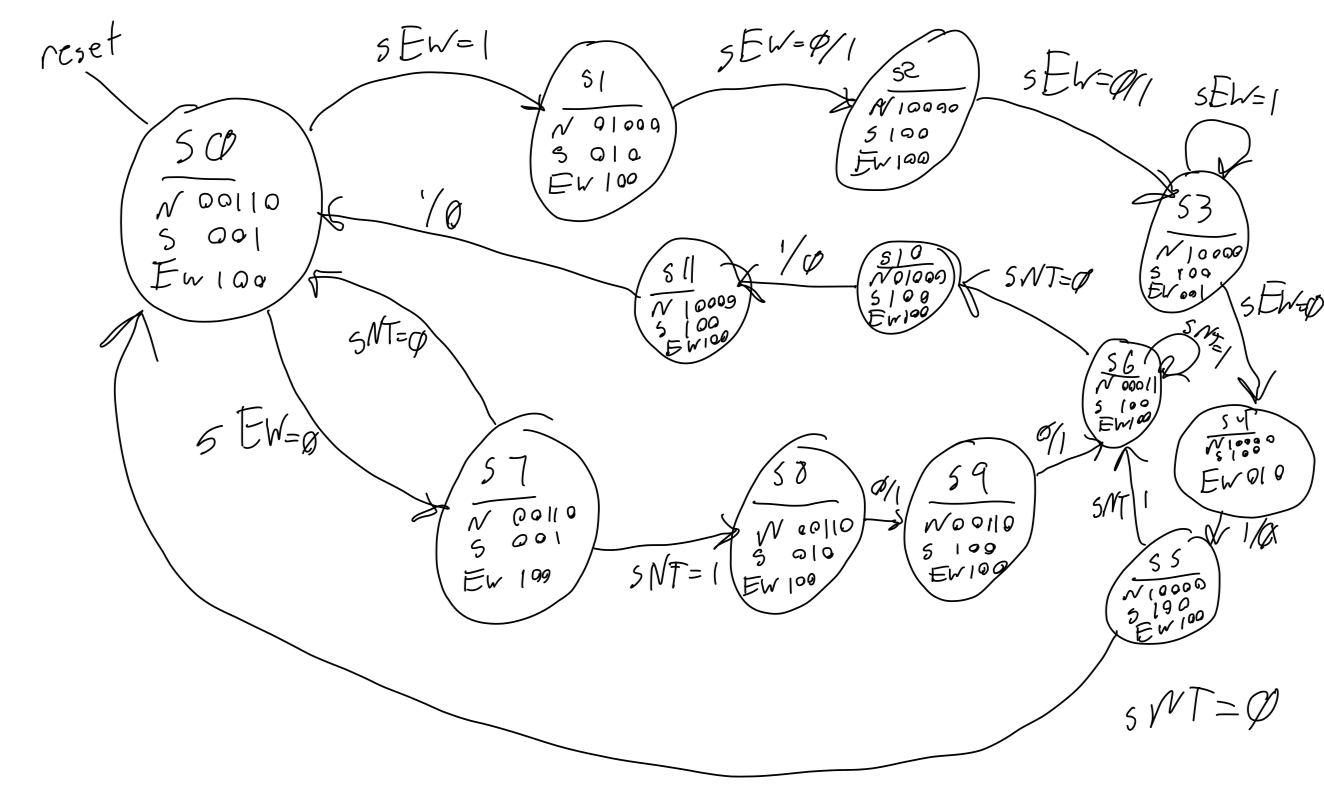
\includegraphics[width=\textwidth]{./9images/trafficLightWithSensorTurn.png}
	\caption{\label{fig:trafficLightWithSensorTurn}State machine for traffic light with a turn lane and a sensor}
\end{center}
\end{figure}

\section{Conclusion}
Finite state machines are very useful for designing fault-tolerant systems that cycle through a set number of states based on limited inputs from users. We are now able to understand and design such systems.

\end{document}